% =========================================================
% PRB/REVTeX 4.2: insert the following blocks at the indicated
% locations in the manuscript. Figures reside in figures/.
% The interpretation R1=longitudinal and R2=Hall is provisional.
% =========================================================

% Under Results -> Temperature-dependent resistance:
\begin{figure}[t]
\centering
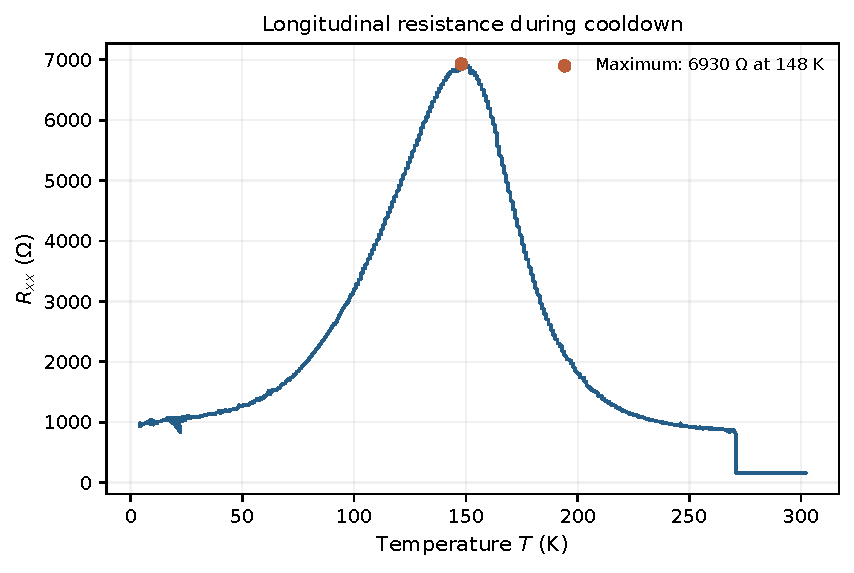
\includegraphics[width=\columnwidth]{figures/fig01_cooldown.pdf}
\caption{Measured SR510 No.~1 resistance during cooling at $B\simeq0$ and $V_g=0$. The maximum is $6930\,\Omega$ near $148\,$K. The signal is a measured resistance, not a geometry-corrected sheet resistivity.}
\label{fig:cooldown}
\end{figure}

% Under Results -> Classical Hall response:
\begin{figure}[t]
\centering
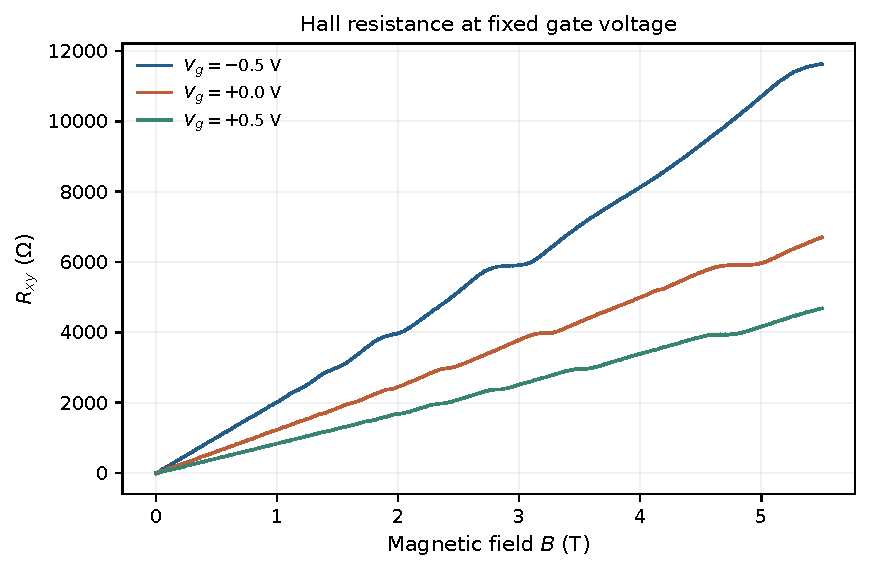
\includegraphics[width=\columnwidth]{figures/fig02_hall_full.pdf}
\caption{Raw SR510 No.~2 resistance versus field at $V_g=-0.5$, $0$, and $+0.5\,$V. The Hall-channel assignment is provisional. The temperature evolves during the field sweeps; high-field features must therefore not be treated as strictly isothermal.}
\label{fig:hall_full}
\end{figure}

\begin{figure}[t]
\centering
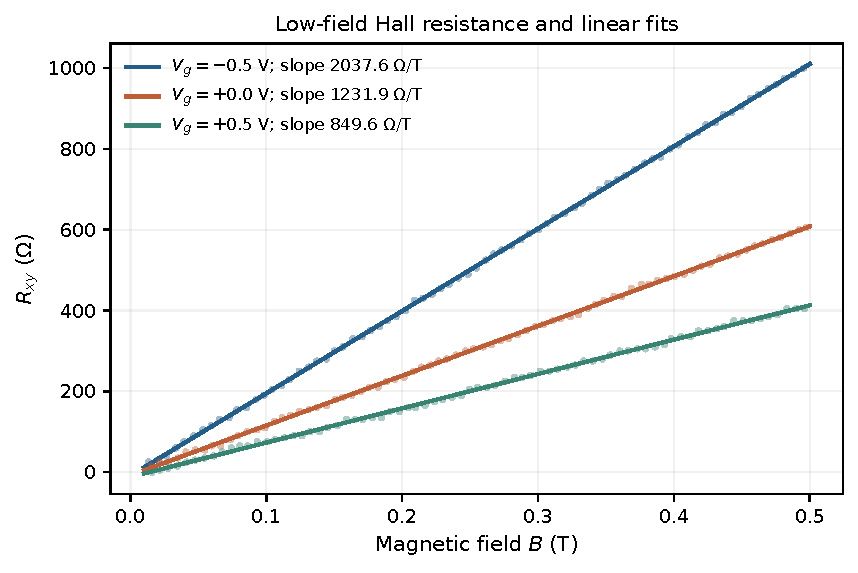
\includegraphics[width=\columnwidth]{figures/fig03_lowfield_fits.pdf}
\caption{Low-field SR510 No.~2 data (symbols) and unconstrained linear least-squares fits (lines) over $0.01\le B\le0.50\,$T. The slopes are $2037.61$, $1231.87$, and $849.63\,\Omega/\mathrm{T}$ at $V_g=-0.5$, $0$, and $+0.5\,$V, respectively.}
\label{fig:hall_fits}
\end{figure}

% Under Results -> Gate-voltage dependence:
\begin{figure}[t]
\centering
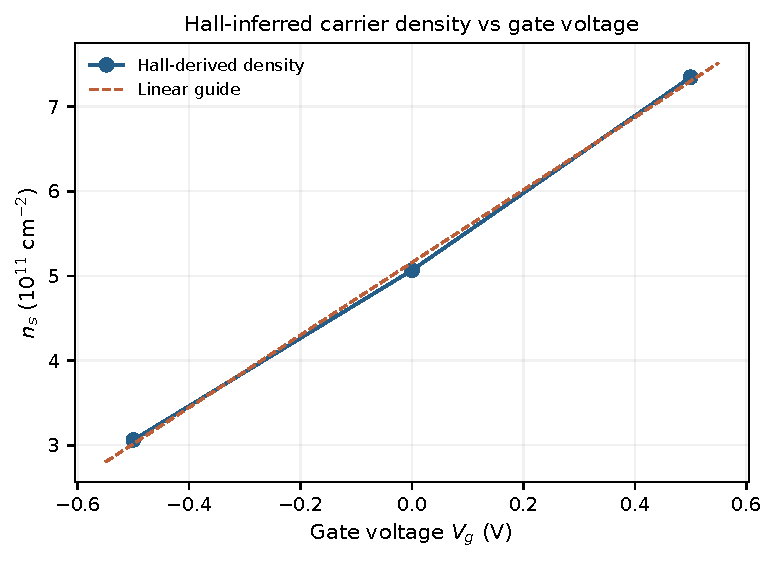
\includegraphics[width=\columnwidth]{figures/fig04_density_vs_gate.pdf}
\caption{Sheet density inferred from the low-field Hall slopes, assuming a single electron carrier population. The dashed line is a guide from a linear regression through the three estimates. The plotted points have no uncertainty bars because the complete systematic error budget has not yet been established.}
\label{fig:gate_density}
\end{figure}

% Under Results -> Magnetotransport at zero gate voltage:
\begin{figure}[t]
\centering
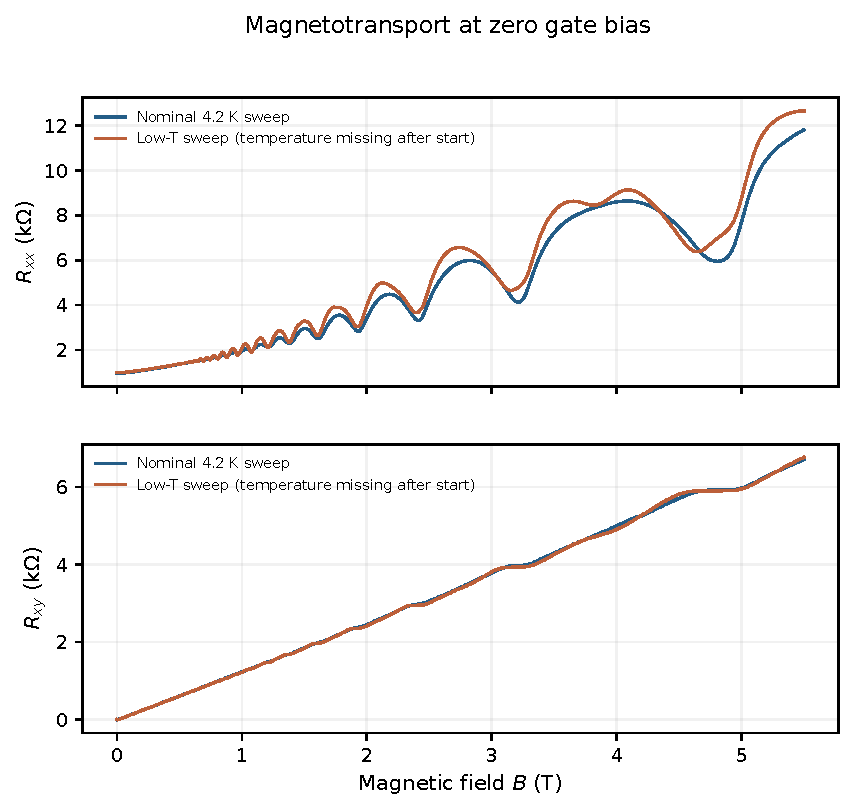
\includegraphics[width=\columnwidth]{figures/fig05_magnetotransport.pdf}
\caption{Comparison of the two resistance channels in field sweeps at zero gate voltage. The standard sweep has temperature drift; the nominally lower-temperature sweep has valid temperature readings only near the beginning. Oscillatory structure is apparent in channel 1, but neither a quantitative SdH frequency nor quantized Hall plateau values have been extracted from this plot.}
\label{fig:magnetotransport}
\end{figure}

% Under Results -> Gate-voltage scans at fixed magnetic field:
\begin{figure}[t]
\centering
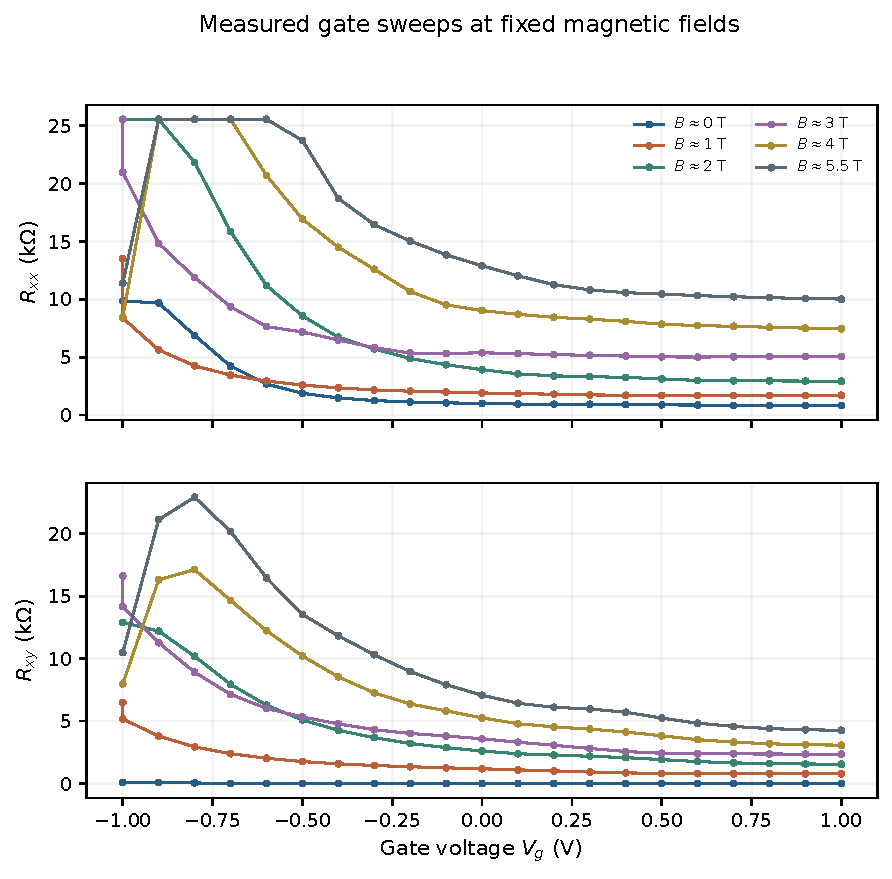
\includegraphics[width=\columnwidth]{figures/fig06_fixed_field_gate.pdf}
\caption{Gate-voltage dependence of both measured SR510 resistance channels for nominal fields $B\simeq0$, $1$, $2$, $3$, $4$, and $5.5\,$T, extracted from the t-series files. Repeated readings of $25565\,\Omega$ near the upper measurement range may represent clipping and must not be used for quantitative fits without checking the instrument setup.}
\label{fig:fixed_field_gate}
\end{figure}

% Under Results -> Gate leakage:
\begin{figure}[t]
\centering
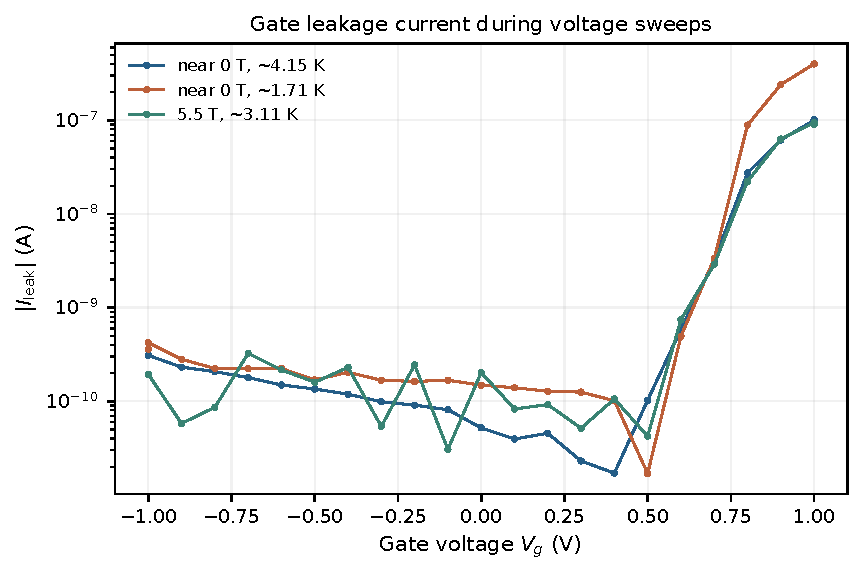
\includegraphics[width=\columnwidth]{figures/fig07_gate_leakage.pdf}
\caption{Magnitude of the recorded gate leakage current versus gate bias for selected fixed-field scans. The substantial increase near positive gate voltages $\gtrsim0.7\,$V should be considered when interpreting gate-capacitance estimates. Absolute values are plotted on a logarithmic scale.}
\label{fig:gate_leakage}
\end{figure}

% Under Results -> Data quality (or Discussion -> Limitations):
\begin{figure}[t]
\centering
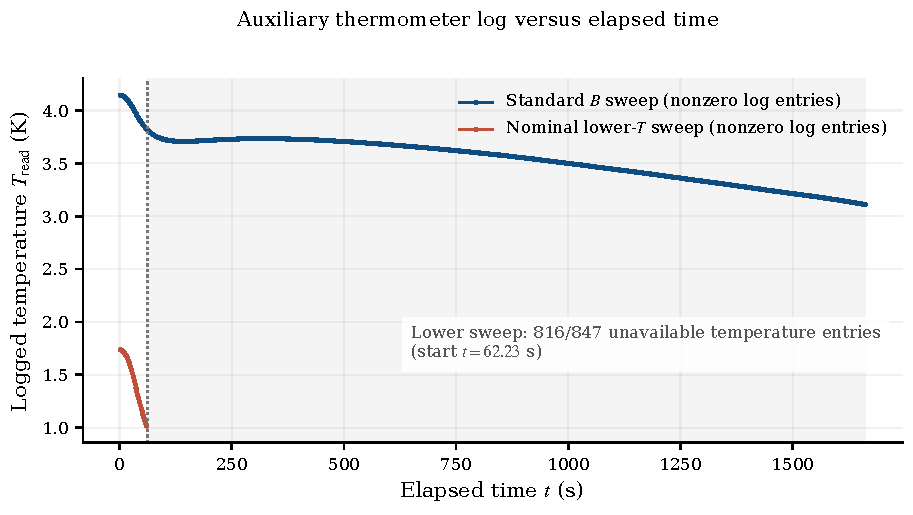
\includegraphics[width=\columnwidth]{figures/fig08_temperature_drift.pdf}
\caption{Recorded temperature during magnetic-field sweeps at $V_g=0$. Zero-valued thermometer entries in the lower-temperature file have been excluded as invalid or missing; hence the lower-temperature curve covers only the start of the scan.}
\label{fig:temperature_drift}
\end{figure}

% Under Results -> High-field gate dependence:
\begin{figure}[t]
\centering
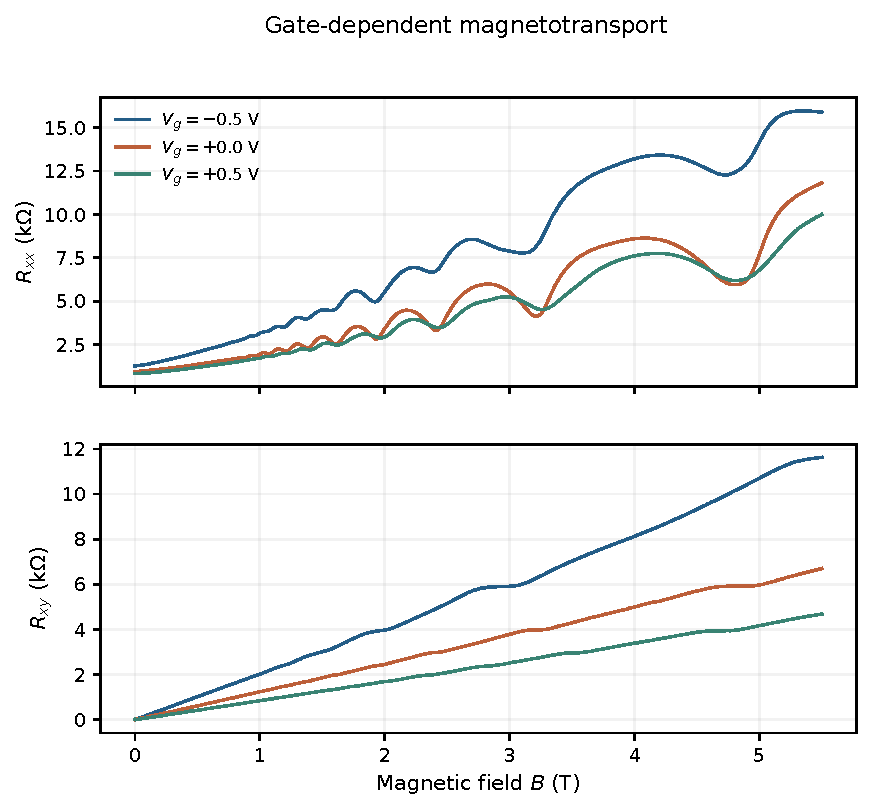
\includegraphics[width=\columnwidth]{figures/fig09_gate_dependent_field.pdf}
\caption{Measured longitudinal-like (SR510 No.~1) and transverse-like (SR510 No.~2) magnetotransport traces at fixed gate voltages. These are raw channel values. Their physical assignment and geometrical calibration should be verified against the sample contact diagram.}
\label{fig:gate_field}
\end{figure}
